\documentclass{article}
\newcommand{\bez}{B\'ezier}
\usepackage{graphicx,xurl,microtype,enumitem,amssymb,amsmath,hyperref}
\title{My Project to Automatically Generate Stitching Instructions of Quadratic \bez\ Curves in Font Files with Python}
\author{John}
\begin{document}
	\maketitle
	{\small This document is licensed under CC BY-SA 4.0 license, in order to comply with the licensing terms of images included.}
	\begin{abstract}
		Over the \(3\) day weekend I was bored and decided to do this.
	\end{abstract}
	
	\section{Intro}
	In string art, quadratic \bez\ curves often appears in designs. Figure~\ref{bezierwikm} shows how it works. The outermost points where the strings intersect are on the quadratic \bez, so it create an illusion of a curve even though it's just a bunch of segments. With a bunch of those curves, they could create complex patterns as illustrated in figure~\ref{actualstrart}. This type of string art, characterized by using straight lines to create the illusions of curves, is also known as curve stitching.
	\begin{figure}\centering
		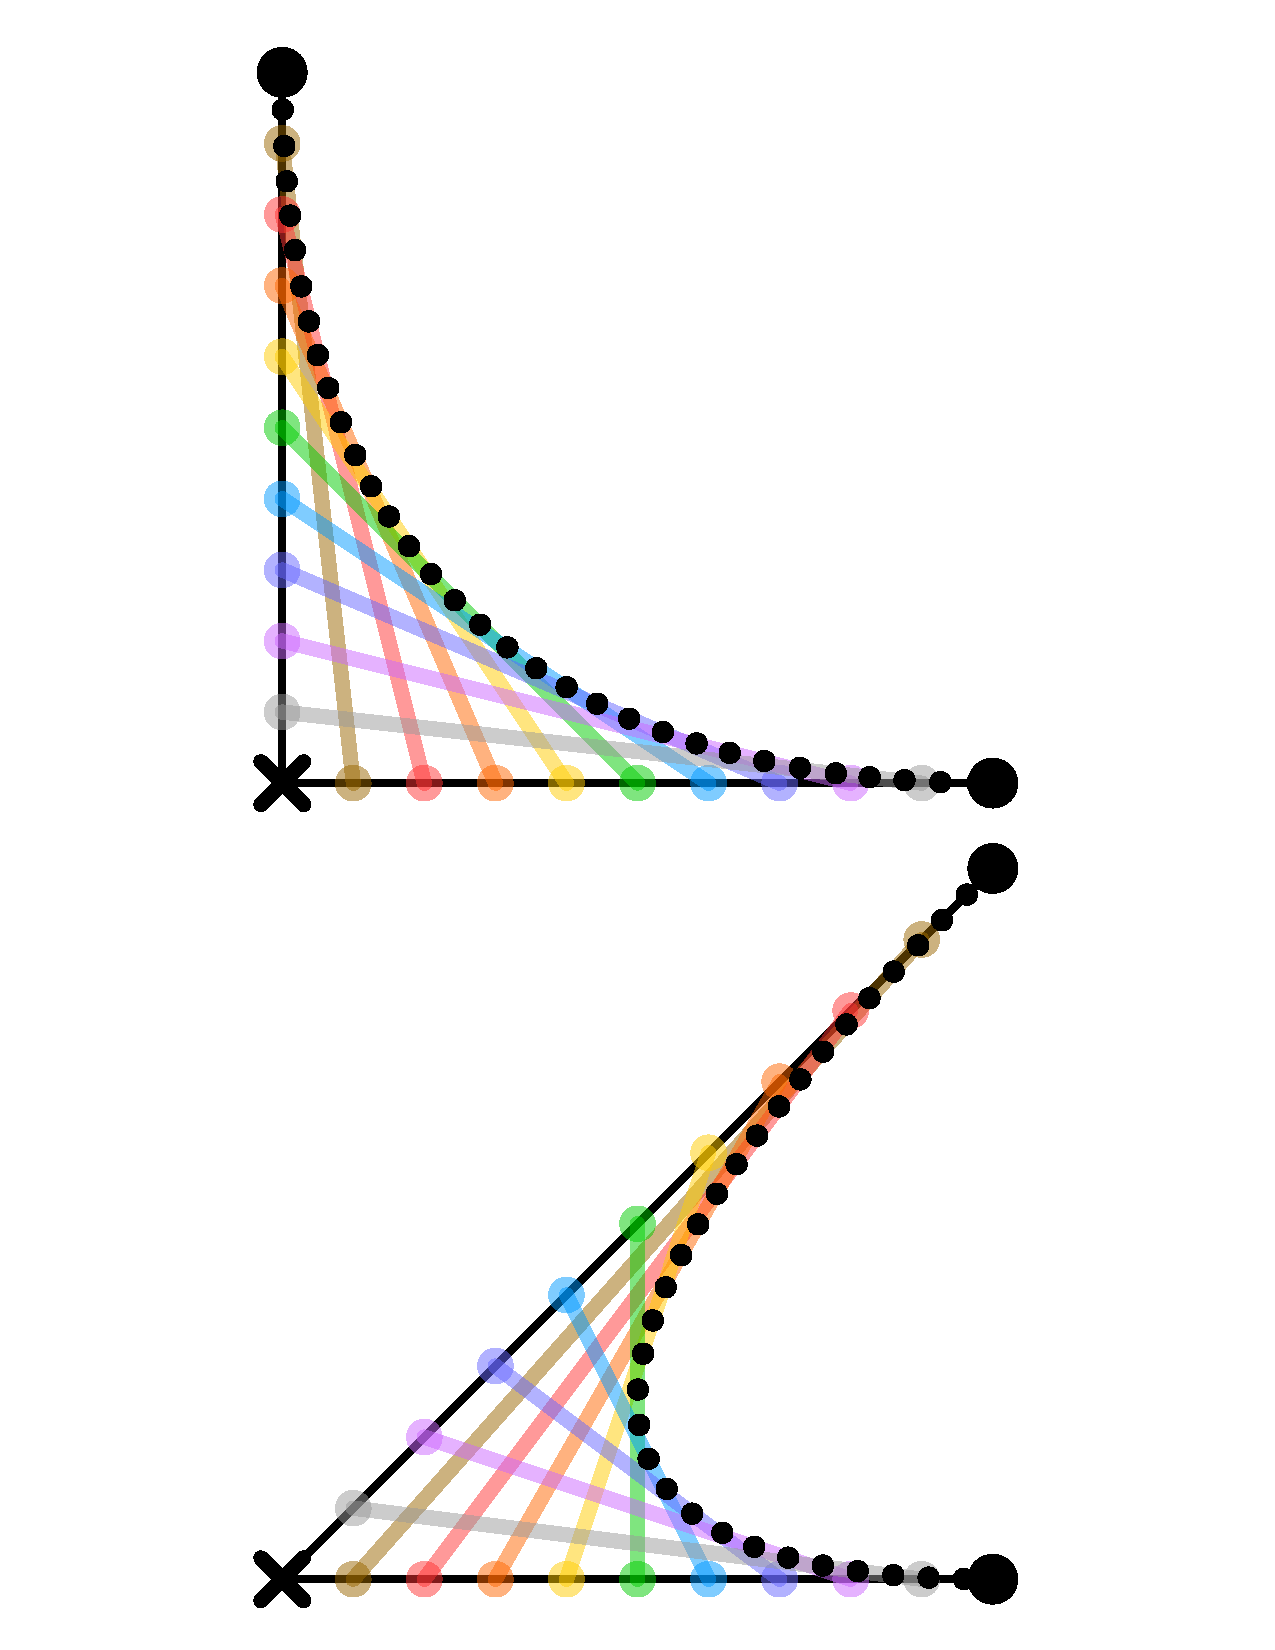
\includegraphics[width=3.3cm]{Quadratic_Beziers_in_string_art.pdf}
		\caption{Quadratic \bez\ curves in String Art. Source: \url{https://commons.wikimedia.org/wiki/File:Quadratic_Beziers_in_string_art.svg}, licensed under CC BY-SA 3.0 license. \label{bezierwikm}}
	\end{figure}
	\begin{figure}\centering
		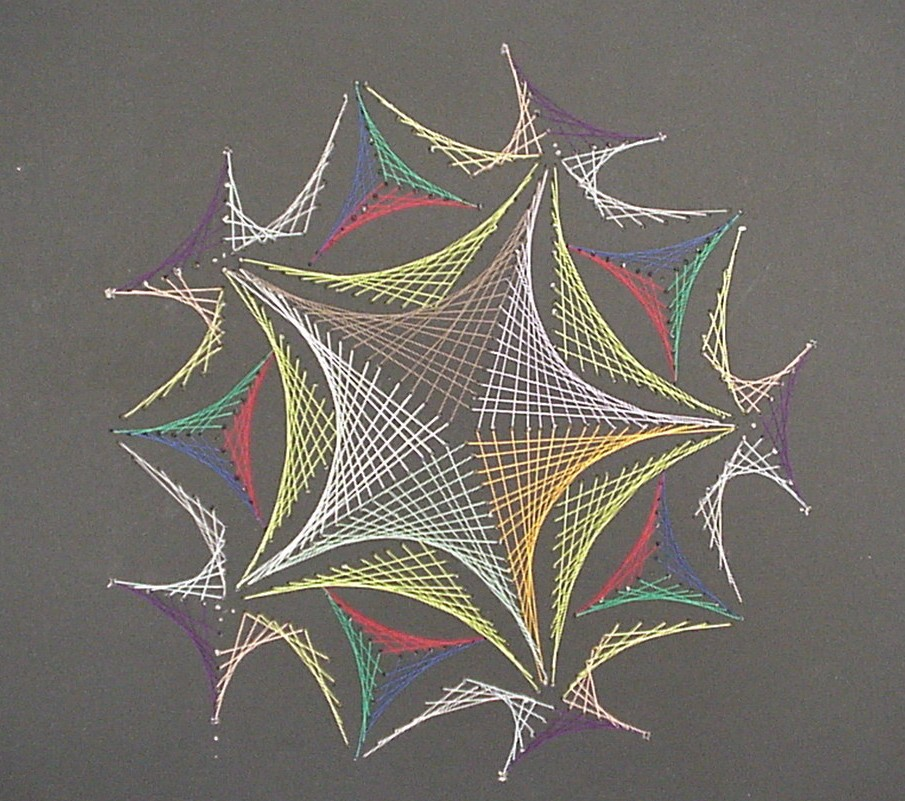
\includegraphics[width=4cm]{StringArt}
		\caption{An example of how quadratic \bez s can get together and create complex patterns. Public domain, from Wikimedia Commons, author unknown.\label{actualstrart}}
	\end{figure}
	
	\bez\ curves were originally developed for automobile design, but when the de~Casteljau's~algorithm, a numerically stable method for evaluating those curves, was invented, they saw increasing use in computer graphics\footnote{Source: \url{https://en.wikipedia.org/wiki/B\%C3\%A9zier_curve}.}. One of such applications are in the way fonts are stored. There are two major types of font formats: PostScript, which uses cubic \bez s, and TrueType, which uses quadratic ones.
	
	Since TrueType font files and flavors of string art both uses quadratic \bez s, it would be possible to stitch those curves in the fonts with string art, as shown in figure~\ref{stitchf}.
	
	\begin{figure}\centering
		\includegraphics[width=4cm]{picture1}
		\caption{Stitching fonts with string art. This is from my final script.\label{stitchf}}
	\end{figure}
	
	\section{General Method}
	I used FontForge to do this task. It's Python API is super helpful. First, to ensure things are quadratic, I first set the \verb|is_quadratic| attribute on the contours; then, I extract all the points and do a bunch of manipulations to extract all the individual \bez s. There were some bugs when FontForge reports the coordinates, but it is mainly fine. This debugging is very tedious as there are a lot of possibilities over the points --- sometimes there is just a straight line, not a control point!
	
	Scripting all that took me around 40 minutes. In the end of that I was able to get a pretty decent-looking result. I introduced a parameter to handle the number of cuts on all sides, and that resulted in crowded areas as shown in figure~\ref{crowded}. We saw some black areas. Also see figure~\ref{crowd2}; notice that small areas looks crowded in cases where we want the overall stuff to be denser. Also there are long curve which would want to have more subdivisions and short ones which should have less.
	\begin{figure}\centering
		\includegraphics[width=4cm]{picture2}
		\caption{First attempt.\label{crowded}}
	\end{figure}
	\begin{figure}\centering
		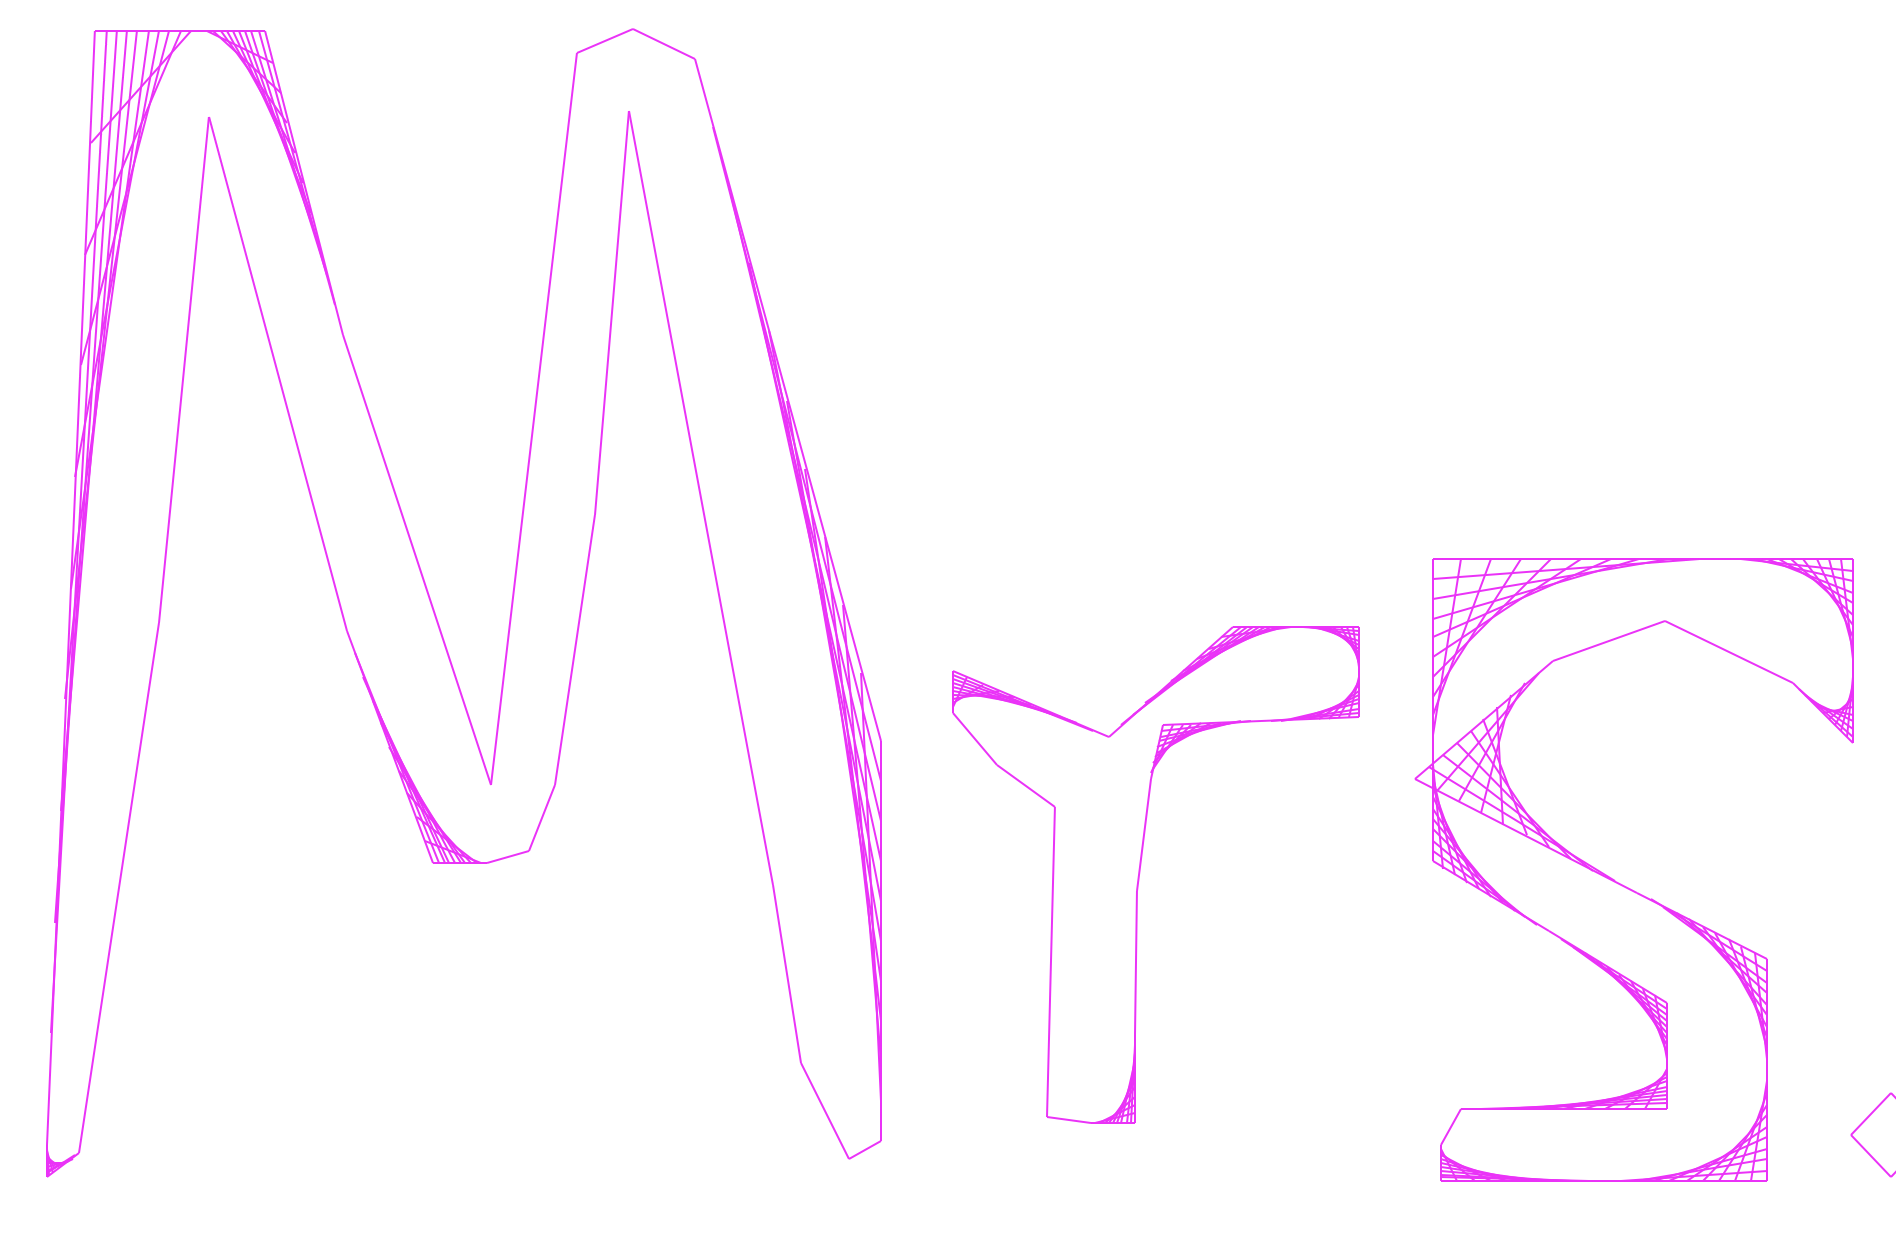
\includegraphics[width=6cm]{bad}
		\caption{First attempt picture number 2. Sorry for the spindly line width.\label{crowd2}}
	\end{figure}
	
	\section{Avoiding Crowded or Light Areas}
	To mitigate this I play around with several factors:
	\begin{itemize}[nosep]
		\item Averaging the handle lengths. Does not really work; too dense when they differ too much.
		\item Square root of averaging handle lengths squared. Works out OK but I'm sure there's a better way.
		\item The area stitched. This is an important factor since you can directly determine how many lines which will dictate how crowded. That fails since I do not know Calculus. Also fails for thin and long areas.
		\item The area between end- and control points. This works partly, except for curves that bends a lot relative to the straight line, and for long and thin curves.
		\item Angle between control handles (\(\arccos\) of a bunch of stuff). It shouts to me, 'I'm a terrible idea!', but I still tried it. Did not work out by itself.
		\item Distance between the control point and the straight line formed by the endpoints. Does not work alone.
	\end{itemize}
	
	After a few more minutes of playing around in Desmos, I was able to recognize some patterns, such as what influences the area. However, there a bunch of factors that plays into deciding how many subdivisions to do. In the end, I came up with a heuristic that seems to work fairly well: Let the points be \(A,B,C\) in which \(A,B\) are the endpoints and \(C\) is the control point. Let a parameter \(a\) decide how much, ideally, should be the spacing. I used \[\mathrm{Subdivs}=2\cdot\frac{S_{\triangle ABC}}{a}\cdot\frac{\text{distance from }C\text{ to }AB}{AB}+\frac{3\sqrt{360-m\angle BCA}\sqrt{AB}}{200}+\frac{AB}{330}\]
	for my heuristic after playing around with a graph I wrote in Desmos. For the angle I looked up a bunch of vector and trig formulas; Google's new ``AI Overview'' feature provided some useful stuff. Note that there might be more implementation details on the above ``formula''.
	
	\section{Finale}
	After that it's just a lot of tweaking. In the end, I was able to get some more than wonderful results. I also implemented outputting string art instructions to a \LaTeX\ file to be compiled into a PDF, and an interactive (well not too interactive) visualization of the stitching with Tkinter. I was not surprised by what I did given all the above effort. You can also see figure~\ref{stitchf} for an example of final output.
\end{document}